\section{Reprodutibilidade}

Reprodutibilidade ({\it reproducibility}) é a habilidade de replicar um
experimento ou estudo em sua totalidade a fim de confirmar suas hipóteses, seja
pelo autor original ou por pesquisadores independentes. Esse conceito é um
ponto central do método científico e tem sido uma preocupação crescente da
comunidade de pesquisa em Engenharia de Software Empírica
\cite{gonzalez_reproducibility_2012}.

A verificação de reprodutibilidade é essencial para a prática do método
científico, pesquisadores reportam seus resultados, que são reforçados à medida
que outros grupos independentes da comunidade científica compartilham
resultados semelhantes \cite{mccormick_itk_2014}. Experimentos são repetidos
com objetivo de checar seus resultados, replicações bem sucedidas aumentam a
validade e confiabilidade dos resultados observados no experimento
\cite{almqvist_replication_2006,juristo_replication_2012}.

Este conceito apesar de ser relativamente concensual entre as várias áreas da
Ciência carece de unidade, inúmeros autores de áreas distintas tem debatido o
tema e proposto terminologias \cite{drummond_replicability_2009,
vitek_repeatability_2011, mendoza_defining_2017, plesser_reproducibility_2018},
segundo \citeonline{feitelson_repeatability_2015} temos as seguintes
definições:

\begin{description}

  \item[Repetição ({\it repetition})]
  Refazer exatamente o que outra pessoa fez usando os artefatos originais.

  \item[Replicação ({\it replication})]
  Replicar com precisão exatamente o que outra pessoa fez, recriando os
  artefatos.

  \item[Variação ({\it variation})]
  Repetir ou replicar exatamente o que a outra pessoa fez, mas com alguma
  modificação controlada nos parâmetros.

  \item[Reprodução ({\it reproduction})]
  Recriar o espírito do que outra pessoa fez, usando seus próprios artefatos.

  \item[Corroboração ({\it corroboration})]
  Obter os mesmos resultados de outra pessoa, usando outros meios e
  procedimentos experimentais.

\end{description}

A comunidade de Engenharia de Software tem tentado por anos replicar
experimentos para gerar fragmentos de conhecimento, mas a grande parte
das tentativas tem levado a resultados insatisfatórios (a
credibilidade dos resultados não aumentou), principalmente por conta das
variações nas condições experimentais de uma replicação para outra
\cite{juristo_using_2009}.

Um estudo com 88 papers da conferência {\it MSR (Mining Software
Repositories)\footnote{\url{http://msrconf.org}}} entre 2004-2011 evidenciou
que apenas 62\% são replicáveis ou parcialmente replicáveis e que apenas 20\%
dos estudos disponibilizam suas ferramentas \cite{amann2015software}. Um estudo
anterior com 171 papers do MSR evidenciou que, entre outros problemas, a
maioria não disponibiliza publicamente as ferramentas e {\it scripts}, mesmo
quando os autores explicitamente afirmam que construíram algo
\cite{robles2010replicating}, apenas 2 entre 154 estudos experimentais
avaliados fornecem os dados e ferramentas necessárias para replicação e
futuras pesquisas \cite{barr_shoulders_2010}.

Esta dificuldade em atingir reprodutibilidade
em estudos científicos baseados em métodos computacionais tem
levado a sérios erros em resultados publicados na literatura acadêmica
\cite{hinsen_activepapers_2015}. O número de repetições apesar de ter crescido nos últimos
anos ainda é muito pequeno, especialmente
considerando a amplitude de tópicos em Engenharia de Software
\cite{silva_replication_2011, kitchenham_evidence-based_2015}.

Em muitos campos científicos onde software tem se tornado ferramenta
fundamental para capturar e analisar dados, este requerimento por
reprodutibilidade implica que plataformas de software e ferramentas confiáveis
e compreensíveis devem estar disponíveis para a comunidade científica
\cite{mccormick_itk_2014}. No entanto, ainda vemos o seguinte questionamento a
respeito dos artefatos de software em pesquisas da Ciência da Computação:
``Onde está o software nas pesquisas sobre linguagem de programação?''
\cite{krishnamurthi_real_2015}.

Toda pesquisa que possua qualquer processo computadorizado deve publicar seus
códigos, eles precisam estar disponíveis, mesmo que os dados correspondentes
não estejam. De acordo com o espectro de reprodutibilidade (Figura
\ref{reproducibility-spectrum}), a disponibilidade de código é o requisito
mínimo e é o primeiro passo para possibilitar validação e confirmação dos
resultados \cite{peng2011reproducible}.

\begin{figure}[h]
  \center
  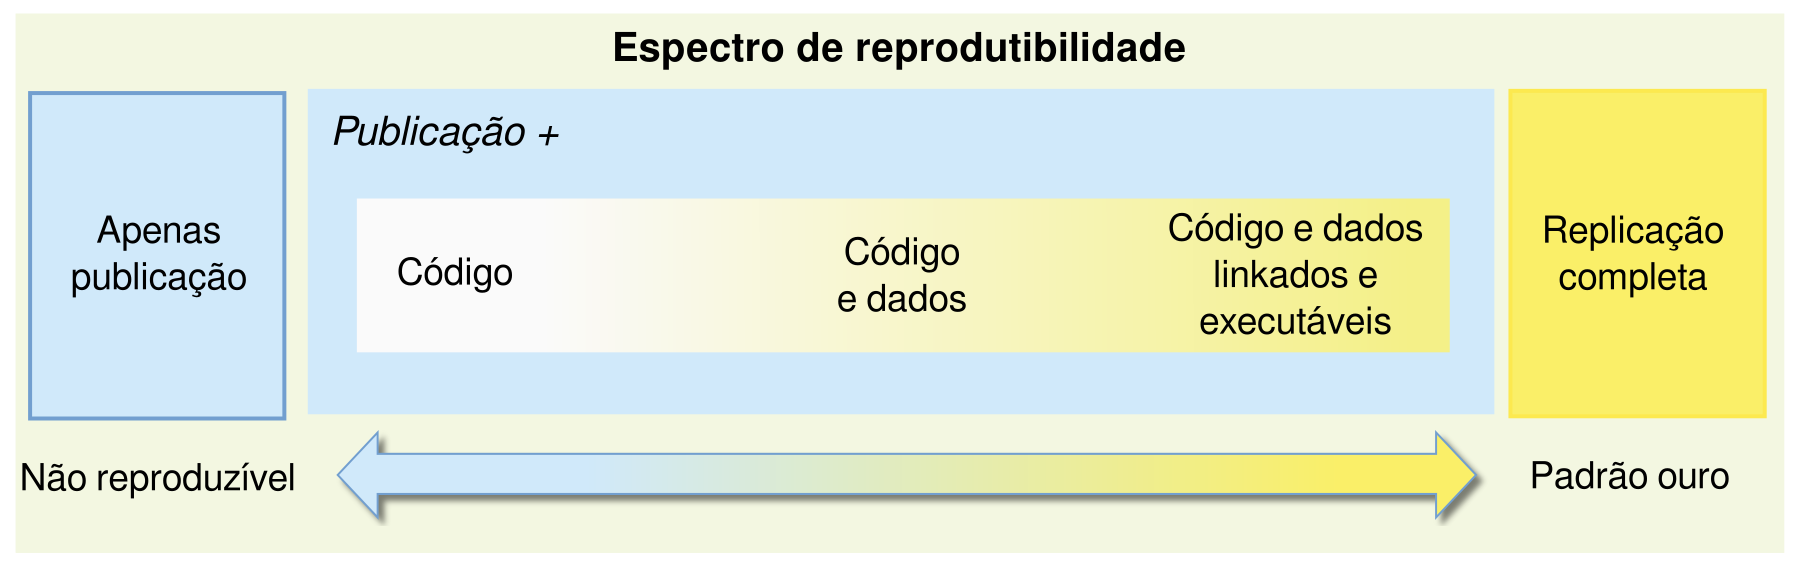
\includegraphics[scale=0.3]{imagens/reproducibility-spectrum-ptbr.png}
  \caption{Espectro de reprodutibilidade \cite{peng2011reproducible}}
  \label{reproducibility-spectrum}
\end{figure}

No entanto, esta prática ainda carece de maior adoção, as questões por trás
destes problemas são, além de outros, possivelmente, ocasionados por questões
culturais, como, por exemplo, a tímida adoção de práticas da ciência aberta
entre pesquisadores \cite{niemeyer2017open}.

\subsection{Ciência Aberta}

Ciência Aberta é um movimento que tem por objetivo tornar a pesquisa
científica, seus dados e sua disseminação acessíveis à todos os interessados,
sejam amadores ou profissionais \cite{WikipediaOpenScience}. Sua principal
motivação está em possibilitar a reprodução dos resultados de pesquisas e em
garantir transparência das metodologias utilizadas, isto aumenta o impacto
social das pesquisas e gera economia de tempo e dinheiro para os pesquisadores
e para as instituições \cite{nesta2010open}.

Este movimento é guiado por princípios básicos de transparência, acessibilidade
e reusabilidade universais, disseminados por ferramentas {\it online}, ele é
dividido em quatro grandes áreas \cite{pontika_fostering_2015}:

\begin{enumerate}
  \item {\it Open Access}.
    Resultados acadêmicos, revisado por pares, disponível {\it online}, de
    maneira livre.

  \item {\it Open Data}.
    Dados coletados durante projetos de pesquisa, disponibilizados {\it
    online} com permissão explícita para uso.

  \item {\it Open Source}.
    Software acessível {\it online}, com código-fonte disponível, com licenças
    que permitam uso, modificação e re-distribuição.

  \item {\it Open Reproducible Research}.
    Ato de aplicar as práticas da Ciência Aberta para permitir reprodutibilidade
    de maneira independente dos resultados de uma pesquisa.
\end{enumerate}

A Ciência Aberta pode ter praticada tanto por razões filosóficas quanto
pragmáticas, os recursos produzidos por projetos abertos são acessíveis ao
público, oferecendo um meio inovador para o envolvimento de terceiros no
processo de Ciência, além de ser um método inovador para comunicação científica
em tempo real \cite{grand_open_2010}.

%A Open Science é uma abordagem emergente para a condução de projetos de
%ciência, tecnologia e engenharia, em que informações sobre toda a pesquisa em
%andamento estão disponíveis e através da Internet. Adotar uma Abordagem de
%Ciência Aberta significa que a audiência para a pesquisa pode se estender além
%dos estudiosos envolvidos para outros pesquisadores e para os membros do
%público. Assim, a Open Science tem implicações para pesquisa de engenharia,
%prática, publicação e engajamento público com engenharia
%\cite{grand_open_2010}.

%I describe my views on why open science practices
%are important (supported by relevant studies), and discuss the po-
%tential societal impact of increased openness
%
%Importância das práticas de Ciência Aberta segundo \citeonline{niemeyer2017open}:
%
%Disponibilidade:
%
%é particularmente importante para o público financiador da pesquisa de forma que
%pesquisas com financiamento público disponibilizem publicamente seus resultados.
%
%Reprodutibilidade:
%
%disponibilizar os produtos da pesquisa, incluindo software e dados ajuda
%a habilitar reprodutibilidade.
%
%Impacto:
%
%Pesquisas abertas aumentam o impacto do trabalho, estudos tem mostrado que artigos
%open-access são mais citados na maioria dos campos científicos, em campos específicos
%o mesmo é notado em open-data e open-source.

